% !TEX root = ../main.tex
\chapter{Related Work} \label{ch:reated_work}

In this chapter, we give an overview of graph based algorithms
for image segmentation 

\section{Multicut}\label{sec:rw_multicut}

Segmentation is an important problem in computer vision as a first step
towards understanding an image. Many algorithms start with an over-segmentation
into superpixels, which are then clustered into ``perceptually meaningful''
regions.
Usually, the number of these regions is not known beforehand.

Recently, the multicut formulation~\cite{chopra_1993_mp}
(sometimes called \emph{correlation clustering}, \cite{bansal_2004_ml})
has become increasingly popular for unsupervised
image segmentation.
Given an edge-weighted region adjacency graph,
the problem is to find the segmentation which
minimizes the cost of the cut edges.
Such an approach has been shown to yield
state-of-the-art results on the Berkeley Segmentation Database
%TODO: - alush_2013_simbad apply it on BSD500, is is state-of-the-art?
%      - gPb-owt is not really learned? Do we need to say this????
\cite{andres_2011_iccv,yarkony_2012_eccv,alush_2013_simbad}.


In this section we will motivate the multicuts and show the basic problem formulation.
In \cref{ch:cgc} we will give an more detailed overview of different solvers
for the multicut objective and introduce a new approximative solver. 


\section{Hierarchical Clustering}\label{sec:rw_hc}

Hierarchical clustering techniques have been successfully used
in computer vision since decades \citep{ohlander_1978_cgip,forsyth_2002_book,arbelaez_2006_cvpr,iglesias_2013,morel_1995_book}.

The method  of \citet{ohlander_1978_cgip} is an example for \emph{top-down} clustering,
where all pixel start in one single cluster. Each cluster is recursively divided 
into  more clusters. The method proposed in \cref{ch:cgc} has a strong connection to
\emph{top-down} clustering.
\citet{arbelaez_2006_cvpr} and \citet{iglesias_2013} use the bottom-up approach 
also called \emph{agglomerative clustering}, where 
adjacent nodes in a graph are merged iteratively to create 
a set of nested segmentations.


Such a hierarchy of clusters can be visualized as a dendrogram (see \cref{fig:hc_bottom_up_top_down} ).
The dendrogram can be interpreted as a tree where each node represents a
region in the image.
The leafs in the tree are the atomic units of the image (e.g. pixel,superpixels, supervoxel)
and the root note is the entire scene itself (e.g. the complete image / graph).

There are a few difference between classic unstructured agglomerative clustering
\citep{florek_1951,sokal_1958_science_bulletin,ward_63_jasa}
and agglomerative clustering on graph data structures \citep{arbelaez_2006_cvpr,iglesias_2013,morel_1995_book}, 
e.g. grid-graphs and region adjacency graphs\citep{vlachos_1993_csv}.
While in unstructured hierarchical clustering any pair of observations could be merged,
in the case of graph hierarchical clustering only adjacent nodes / regions can be merged.
In the literature this is also called ``hierarchical clustering with connectivity constraints''.


The main idea behind agglomerative clustering is very simple:

Initially, all observations start in a single cluster. 
Next, cluster which have highest similarities / lowest distances will be merged.
Due to the merging, similarities will change and need to be updated
/ recomputed. Therefore  noisy initial features
will  become more informative .

The definition of a specific distance betweens clusters is very crucial, 
but does strongly depend on the application.
In \cref{tab:hc_distance_types} is a short overview of most common distance
types and in   \cref{tab:hc_linkage_types} is a  brief overview 
of cluster distance linkage types.








\iffalse
\begin{tikzpicture}[scale=  1,every node/.style={minimum size=1cm},on grid]
        
    %slanting: production of a set of n 'laminae' to be piled up. N=number of grids.
    

    %%%%%%%%%%%%%%%%%%%%%%%%%%%%%%%%%%%%%%%%%%%%%%%%%%%%%%%%%%%%%%%
    % 0 bottom layer
    %%%%%%%%%%%%%%%%%%%%%%%%%%%%%%%%%%%%%%%%%%%%%%%%%%%%%%%%%%%%%%%%
        
    \begin{scope}[yshift=0,every node/.append style={yslant=0.5,xslant=-1},yslant=0.5,xslant=-1]
        \draw[-latex,thick] (-0.17,3.21/2) node[right]{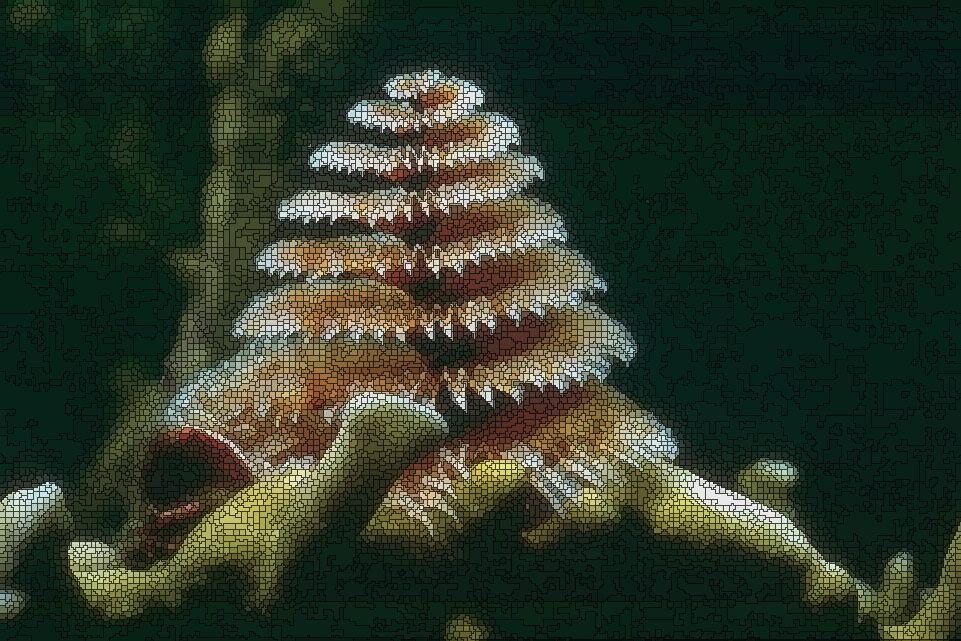
\includegraphics[width=4.82cm]{fig/12074/0.png}};
        \draw[black,very thick] (0,0) rectangle (4.81,3.21);
    \end{scope}

    \begin{scope}[yshift=60*1,every node/.append style={yslant=0.5,xslant=-1},yslant=0.5,xslant=-1]
        \draw[-latex,thick] (-0.17,3.21/2) node[right]{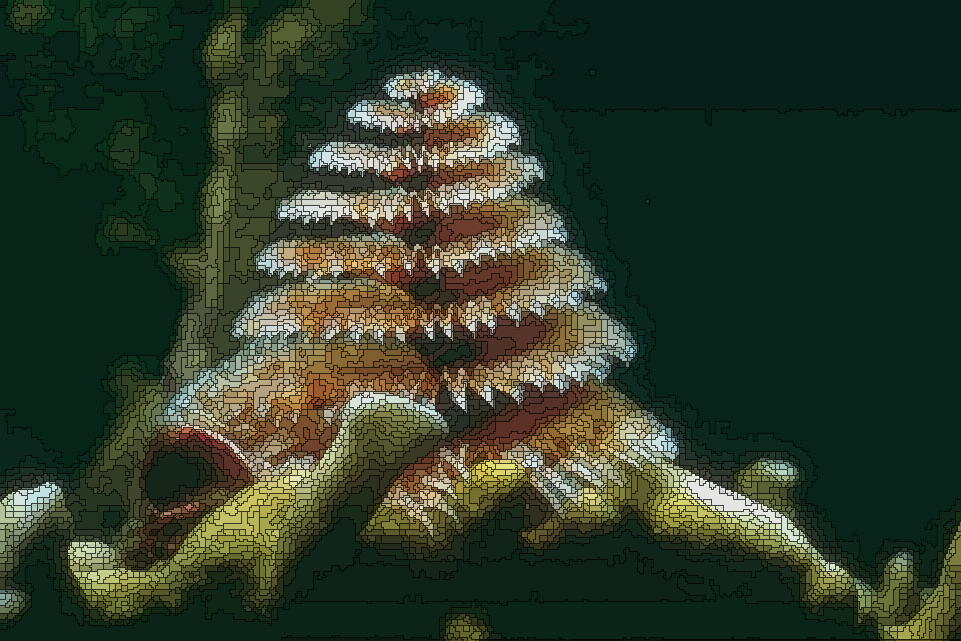
\includegraphics[width=4.82cm]{fig/12074/2.png}};
        \draw[black,very thick] (0,0) rectangle (4.81,3.21);
    \end{scope}

    \begin{scope}[yshift=60*2,every node/.append style={yslant=0.5,xslant=-1},yslant=0.5,xslant=-1]
        \draw[-latex,thick] (-0.17,3.21/2) node[right]{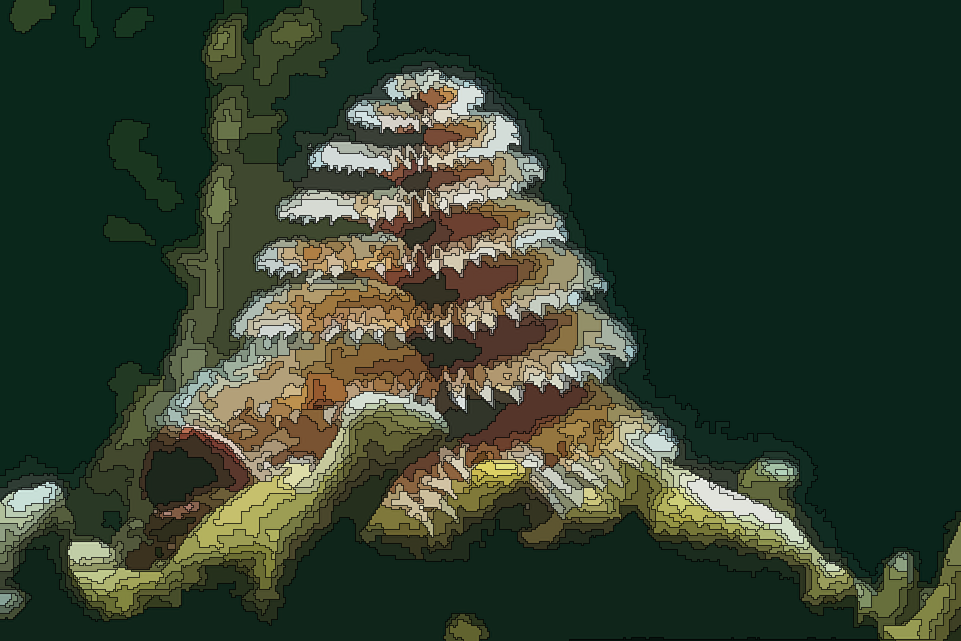
\includegraphics[width=4.82cm]{fig/12074/4.png}};
        \draw[black,very thick] (0,0) rectangle (4.81,3.21);
    \end{scope}

    \begin{scope}[yshift=60*3,every node/.append style={yslant=0.5,xslant=-1},yslant=0.5,xslant=-1]
        \draw[-latex,thick] (-0.17,3.21/2) node[right]{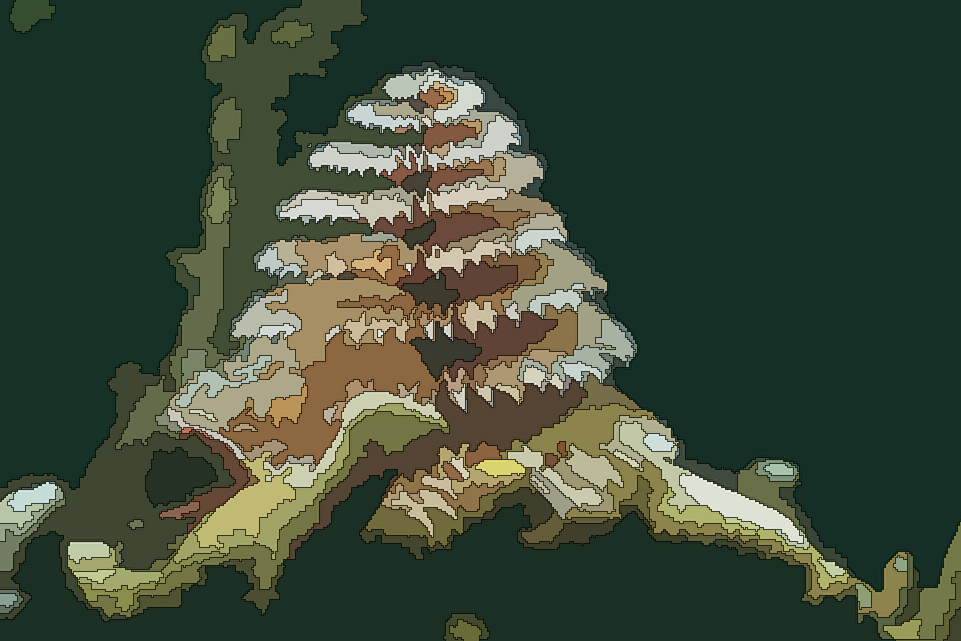
\includegraphics[width=4.82cm]{fig/12074/6.png}};
        \draw[black,very thick] (0,0) rectangle (4.81,3.21);
    \end{scope}

    \begin{scope}[yshift=60*4,every node/.append style={yslant=0.5,xslant=-1},yslant=0.5,xslant=-1]
        \draw[-latex,thick] (-0.17,3.21/2) node[right]{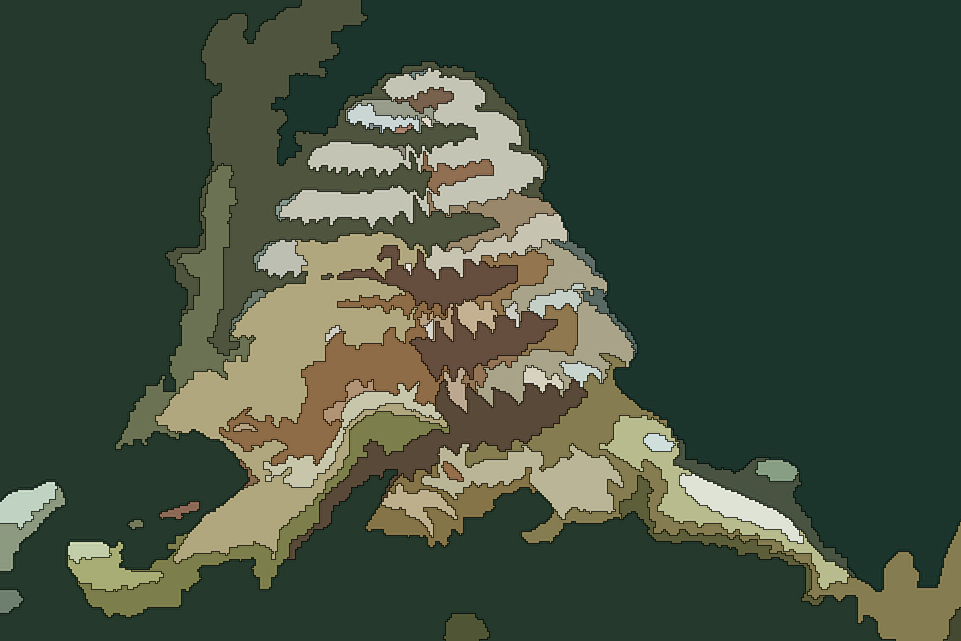
\includegraphics[width=4.82cm]{fig/12074/8.png}};
        \draw[black,very thick] (0,0) rectangle (4.81,3.21);
    \end{scope}


    \draw[->,-triangle 60] (-3,0) -- node[above]{time} (-3,4);

    %%%%%%%%%%%%%%%%%%%%%%%%%%%%%%%%%%%%%%%%%%%%%%%%%%%%%%%%%%%%%%%
    % 0 bottom layer
    %%%%%%%%%%%%%%%%%%%%%%%%%%%%%%%%%%%%%%%%%%%%%%%%%%%%%%%%%%%%%%%%
    \draw[-latex,thick] (6.2,2) node[right]{$\mathsf{over-segmentation}$}
         to[out=180,in=90] (4,2);
         
         
         
    %%%%%%%%%%%%%%%%%%%%%%%%%%%%%%%%%%%%%%%%%%%%%%%%%%%%%%%%%%%%%%%
    % 1 layer
    %%%%%%%%%%%%%%%%%%%%%%%%%%%%%%%%%%%%%%%%%%%%%%%%%%%%%%%%%%%%%%%%
    
    \draw[-latex,thick] (6.2,5.5) node[right]{$\mathsf{Region adjacency graph 1}$}
         to[out=180,in=90] (4,5.5);
\end{tikzpicture}
\fi

\begin{figure}
    \centering
    \subfloat[Bottom-Up: Nodes are merged with increasing time]{\label{fig:hc_bottom_up}
        {
            \begin{tikzpicture}[sloped]
                \node (a)    at (-6,0)      {a};
                \node (b)    at (-5,0)      {b};
                \node (c)    at (-4,0)    {c};
                \node (d)    at (-3,0)     {d};
                \node (e)    at (-2,0)       {e};

                \node (ab)   at (-5.5,1)    {};
                \node (cd)   at (-3.5,1)    {};
                \node (cde)  at (-2.75,2)       {};
                \node (all)  at (-4,3)    {};
                
                \node (root) at (-4,4) {root}; 

                \draw (a) |- (ab.center);
                \draw (b) |- (ab.center);
                \draw (c) |- (cd.center);
                \draw (d) |- (cd.center);
                \draw (e) |- (cde.center);
                \draw (cd.center) |- (cde.center);
                \draw (ab.center) |- (all.center);
                \draw (cde.center) |- (all.center);
                \draw (all.center) |- (root.center);

                \draw[->,-triangle 60] (-7,0) -- node[above]{time} (-7,4);
            \end{tikzpicture}
        }
    }\hspace{2cm}
    \subfloat[Top-Down: Nodes are divided with increasing time]{\label{fig:hc_top_down}
        {
            \begin{tikzpicture}[sloped]
                \node (a)    at (-6,0)      {a};
                \node (b)    at (-5,0)      {b};
                \node (c)    at (-4,0)    {c};
                \node (d)    at (-3,0)     {d};
                \node (e)    at (-2,0)       {e};

                \node (ab)   at (-5.5,1)    {};
                \node (de)   at (-2.5,1)    {};
                \node (cde)  at (-3.25,2)       {};
                \node (all)  at (-4,3)    {};
                
                \node (root) at (-4,4) {root}; 

                \draw (a) |- (ab.center);
                \draw (b) |- (ab.center);
                \draw (c) |- (cde.center);
                \draw (d) |- (de.center);
                \draw (e) |- (de.center);        
                \draw (de.center) |- (cde.center);
                \draw (ab.center) |- (all.center);
                \draw (cde.center) |- (all.center);
                \draw (all.center) |- (root.center);

                \draw [->,-triangle 60] (-7,4) -- node[below,align=center]{time} (-7,0);
            \end{tikzpicture}
        }
    }
    \caption{
        Describe the difference between both
    }
    \label{fig:hc_bottom_up_top_down}
\end{figure}






In the case of graph hierarchical clustering, informative features
can also be attached to the edges of the graph.
Unsupervised edge detectors as gPb \citep{marie_2008_cvpr}  or learned
edge detectors \cite{dollar_2013_iccv}  can be used to boost performance
of agglomerative clustering.









\begin{table}
\begin{scriptsize}
\begin{tabular}{ |l|l|p{5cm}|}
    \hline 
    Euclidean Distance
        & $||a-b||_2 = \sqrt{\sum{ (a_i-b_i })^2 } $
        & For low dimensional data \\  \hline 
    Squared Euclidean Distance
        & $||a-b||_2^2 = \sum{ (a_i-b_i })^2  $
        & For low dimensions data\\  \hline
    Manhattan Distance
        &  $||a-b||_1 = \sum{ |a_i-b_i |}  $
        & Multi purpose \\  \hline 
    Mahalanobis Distance 
        & $\sqrt{(a-b)S^-1(a-b)^T}$
        & ??? when to use \\  \hline 
    $\mathcal{X}^2$-Distance  
        &  $\frac{1}{2}\sum{  \frac{(a_i-b_i)^2}{a_i+b_i} }$
        & For histograms \\  \hline 
    Earth Mover  Distance          
        &  see \citet{levina_2001_iccv} 
        & For histograms \\  \hline 

\end{tabular}

\end{scriptsize}
\caption{
    An overview of the most common distances measurements and their main properties.
}\label{tab:hc_distance_types}
\end{table}



\begin{table}
\begin{scriptsize}
\begin{tabular}{ |l|l|p{5cm}|}
    \hline
    Average Linkage \citep{sokal_1958_science_bulletin}           
        & $d_{al}(C_a,C_b) = \frac{1}{|C_a||C_b|} \sum _{a \in C_a} \sum_{b \in C_b} d(a,b) $ 
        & \scriptsize Prefers clusters with same variance \cite{sokal_1958_science_bulletin} \\ \hline

    Single Linkage \citep{florek_1951}            
        & $d_{sl}(C_a,C_b) =  \min\{d(a,b) : a \in C_a, b \in C_b\}$ 
        & Nice theoretic properties \citep{hartigan_1981_jjamstat,milligan_1980_psycho}, can lead
          to very irregular shaped clusters \\ \hline
    Complete Linkage \citep{sorensen_1948}         
        & $d_{cl}(C_a,C_b) =  \max\{d(a,b) : a \in C_a, b \in C_b\}$ 
        & Prefers clusters with same diameter \citep{milligan_1980_psycho} \\ \hline
    Centroid Distance         
        & $d_{cd}(C_a,C_b) =  d(\bar{C}_a,\bar{C}_b) $ 
        & Robust w.r.t. outliers \citep{milligan_1980_psycho} \\ \hline
    Wards Minimum Variance \citep{ward_63_jasa}
        & $d_{wmv}(C_a,C_b) = \frac{ d(\bar{C}_a,\bar{C}_b)}{ \frac{1}{|C_a|} + \frac{1}{|C_b|} } $ 
        & Prefers clusters with same size, is sensible to outliers \citep{milligan_1980_psycho} \\ \hline
\end{tabular}

\end{scriptsize}
\caption{
    An overview of the most common cluster distances linkages and their main properties.
}\label{tab:hc_linkage_types}
\end{table}






\begin{figure}  \label{fig:ucm_visu}
    \begin{center}
        \subfloat[$K_0$]{ \label{fig:ucm_k0}
            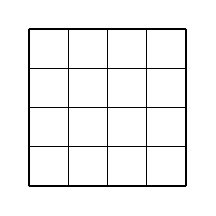
\begin{tikzpicture}
                \draw[step=0.5,black,thin] (0.0,0.0) grid (2,2);
                \draw[step=2,black,thick] (0.0,0.0) grid (2,2);
            \end{tikzpicture}
        }
        \hspace{0.5cm}
        %
        %
        %
        \subfloat[$K_1$]{ \label{fig:ucm_k1}
            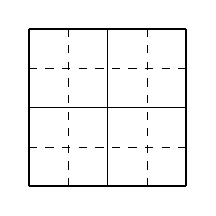
\begin{tikzpicture}
                \draw[step=0.5,black,very thin,dashed] (0.0,0.0) grid (2,2);
                \draw[step=1,black,thin] (0.0,0.0) grid (2,2);
                \draw[step=2,black,thick] (0.0,0.0) grid (2,2);
            \end{tikzpicture}
        }
        \hspace{0.5cm} 
        %
        %
        %
        \subfloat[$K_2$]{\label{fig:ucm_k2}
            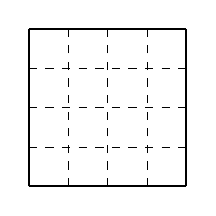
\begin{tikzpicture}
                \draw[step=0.5,black,very thin,dashed] (0.0,0.0) grid (2,2);
                \draw[step=2,black,thick] (0.0,0.0) grid (2,2);
            \end{tikzpicture}
        }
        \hspace{0.5cm}
        %
        %
        %
        \subfloat[$\mathcal{C}(\Upsilon) $]{ \label{fig:ucm_saliency}
            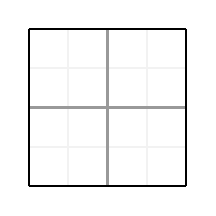
\begin{tikzpicture}
                \draw[step=0.5,black!5,thick] (0.0,0.0) grid (2,2);
                \draw[step=1,  black!40,thick] (0.0,0.0) grid (2,2);
                \draw[step=2,black,thick] (0.0,0.0) grid (2,2);
            \end{tikzpicture}
        }
        \hspace{0.5cm}
        %
        %
        %
        \subfloat[$\mathcal{C}(\Upsilon) $]{ \label{fig:ucm_saliency_3d}
            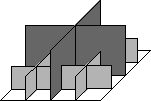
\includegraphics[width=0.2\textwidth]{fig/ucm3d.pdf}
        }
    \end{center}
    \caption{
        \Cref{fig:ucm_k0} shows the an $4x4$ grid graph which servers as initial segmentation $K_0$.
        \Cref{fig:ucm_k1} shows the segmentation $K_0$ after the contraction of a few edges.
        Contracted edges are showed dashed.
        \Cref{fig:ucm_k2} shows the graph after all edges have been contracted.
        \Cref{fig:ucm_saliency} shows the saliency $\mathcal{C}$ of the contour $\Upsilon$ of the contours.
        In \cref{fig:ucm_saliency_3d} the saliency from \ref{fig:ucm_saliency} as a 3D visualization.
        This figure is very much inspired from a figure showed in \citep{arbelaez_2006_cvpr}.
    }
\end{figure}











\subsubsection{Ultrametric Contour Map}\label{sec:hc_ucm}

A generic framework for boundary extraction and image segmentation based
on bottom-up hierarchical clustering, named Ultrametric Contour Map (UCM), 
has been proposed by \citet{arbelaez_2006_cvpr} . 
Starting from an over-segmentation, a region adjacency graph (RAG) is set up.
The edges of the RAG are weighted by an edge indicator and therefore a measure  of dissimilarity.
The main idea of UCM is to iteratively contract the edge with the lowest weight, 
and updating the edge weights while doing so.

\section{MST Methods}\label{sec:rw_mst_methods}


Discuss the method from \citet{felzenszwalb_2004_ijcv}.


Discuss the method from \citet{Straehle_k-smallestspanning}.



\section{Watershed Methods}

Discuss the method from \citet{straehle_2011_miccai}


Discuss the method from \citet{straehle_2012_cvpr}

